\chapter{Cores and Flashing}
\label{cha:cores}

\phantomsection
\section{What are Cores, and Why Do They Matter?}

The MEGA65 computer uses a versatile chip called an FPGA as its heart, which is
an acronym for ``Field Programmable Gate Array''. This is a fancy way of
saying that FPGAs are chips that can be programmed {\it by you} to impersonate
other chips. They do this by re-configuring their arrays of logic gates to
reproduce the circuits of other chips. As a result, FPGAs are not an emulation,
but a re-creation of other chips.

However, FPGAs forget what chip they are pretending
to be whenever the power is turned off, or when they are re-programmed.
This might sound annoying, but it's actually very powerful. It means that
you can tell the FPGA in the MEGA65 to impersonate not just the MEGA65 design
as it currently stands, but to impersonate any improvements made to the design itself.
In other words, you can upgrade the MEGA65 hardware just by providing a new
set of instructions to the FPGA.  These sets of instructions are called ``cores'',
or ``bitstreams''. For the purpose of the MEGA65, these two terms are interchangeable.

FPGAs are so flexible that not only is it possible to teach the MEGA65 to be a better
MEGA65, but it is also possible to teach the MEGA65 to be other interesting
home computers. We believe that the FPGA is powerful enough to re-create
a Commodore PET\texttrademark, VIC-20\texttrademark, Apple II\texttrademark, Spectrum\texttrademark,
BBC Micro\texttrademark, or even an Amiga\texttrademark, or one of the 16-bit era game consoles. Unlike some
previous FPGA-based retro-computers, the MEGA65, its FPGA instructions, board layout, and other information is
all available for free under various open-source licenses. This means that anyone is free to
create other cores for the MEGA65 hardware.

To top it all off, the MEGA65 has enough storage for 7 different sets of FPGA instructions,
so that you can easily switch the MEGA65's ``personality'' from being a MEGA65 to another
system, and back again.

The remainder of this chapter describes how to select a core to run on the MEGA65, and
how to store a core into one of the seven slots in the flash memory storage.

\ifdefined\printmanual
% no need for model types to be in the user guide?
\else
  \subsection{Model types}
  Retail models of the MEGA65 are referred to as the MEGA65R3A (revision 3A). Throughout the course of development of the MEGA65, there have been several other model variants used by developers, each with differing specifications and available core slots, so they will be listed here, just to raise awareness of them.

  \begin{minipage}{\linewidth}
    \begin{center}
      \begin{longtable}{|C{2.5cm}|C{2cm}|C{2cm}|C{2cm}|C{2cm}|}
        \hhline{|=|=|=|=|=|}
        {\textbf{Model}} & {\textbf{FPGA type}} & {\textbf{QSPI size}} & {\textbf{\#slots}} & {\textbf{slot size}} \\
        \hhline{|=|=|=|=|=|}
        \multirow{2}{*}{\textbf{MEGA65R3A}} & \multicolumn{4}{l|}{The retail/release version of the MEGA65} \\
        \cline{2-5}
        & A200T & 64MB & 8 & 8MB \\
        \hhline{|=|=|=|=|=|}
        \multirow{2}{*}{\textbf{MEGA65R3}} & \multicolumn{4}{l|}{The DevKit model} \\
        \cline{2-5}
        & A200T & 32MB & 4 & 8MB \\
        \hhline{|=|=|=|=|=|}
        \multirow{2}{*}{\textbf{MEGA65R2}} & \multicolumn{4}{l|}{An earlier MEGA65 model} \\
        \cline{2-5}
        & A100T & 32MB & 8 & 4MB \\
        \hhline{|=|=|=|=|=|}
        \multirow{2}{*}{\textbf{Nexys4}} & \multicolumn{4}{l|}{FPGA development boards used early in the project} \\
        \cline{2-5}
        & A100T & 16MB & 4 & 4MB \\
        \hline
      \end{longtable}
    \end{center}
  \end{minipage}
\fi


\section{Bitstream files}
\label{sec:bitstreamfiles}

Firstly, there are a variety of files related to the MEGA65's cores/bitstreams that you should be familiar with, in
order to decide what file-types are needed for what occasion.

\subsection{File types}

%\index{.bit files}\index{.mcs files}\index{.prm files}\index{.cor files}
\begin{center}
  \begin{longtable}{|L{1.5cm}|p{10cm}|}
    \hline
    {\textbf{File-type}} & {\textbf{Purpose}} \\
    \hline
    {\tt .cor} & {The MEGA65 project's custom bitstream file format, containing extra header information to help identify the bitstream and the specific MEGA65 target device it is intended for. The MEGA65's flashing utility makes use of this additional information to ensure you don't accidentally flash the bitstream of a different device.} \\
    \hline
    {\tt .mcs} & {The bitstream file in a format needed when flashing it to your device's QSPI flash memory chip via Vivado\textregistered.} \\
    \hline
    {\tt .prm} & {This file contains checksum information that can be used by Vivado to verify the {\tt .mcs} file you have tried to flash. Optional.} \\
    \hline
    {\tt .bit} & {A plain bitstream file that can be copied to your SD card.} \\
    \hline
  \end{longtable}
\end{center}

\subsection{Where to Download}

Visit the following url:

\url{https://files.mega65.org}

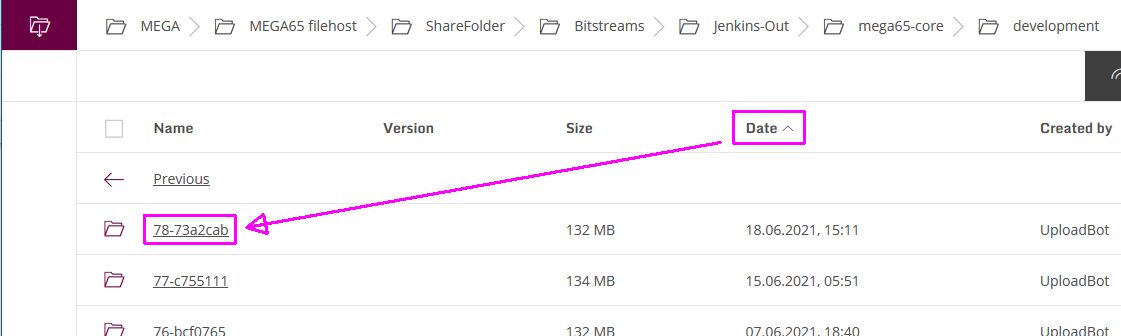
\includegraphics[width=\linewidth]{images/latest_bitstream.png}

Click the {\bf Files} tab, and in the search-bar, type {\bf .cor} and press Enter.
\ifdefined\printmanual
  You will notice that there are different files with the {\tt .cor} extension. For your MEGA65, download the file
  that ends with {\bf 65r3-dev.cor}. Other files are for other device types, which you can read more about in the
  {\bf MEGA65 Book}.
\else
  For the purposes of this chapter on core-flashing, download the desired .cor file that suits your target device:

  \begin{itemize}
    \item{\textbf{mega65r3-dev.cor} (for MEGA65R3 boards, both Release and DevKits)}
    \item{\textbf{mega65r2-dev.cor} (for MEGA65R2 boards)}
    \item{\textbf{nexys4ddr-widget-dev.cor} (for Nexys4 DDR boards)}
    \item{\textbf{nexys4-dev.cor} (for Nexys4 PSRAM boards)}
    \item{You can also find .bit, .mcs and .prm files located here too.}
  \end{itemize}

  Alternatively, if you intend to flash the QSPI chip via Vivado, you would instead download the .mcs file for your target device (and optionally, the .prm files as well).

  Another alternative for Nexys4 board users is to download .bit files and copy them to SD cards, which you can also download.

  But once again, for the purposes of this chapter on core-flashing, you will only be interested in the .cor files.
\fi

\phantomsection
\section{Selecting a Core}

To operate the MEGA65 with an alternate core, switch off the power to the MEGA65, and then hold
\specialkey{NO SCROLL} down while switching the power back on. This instructs the MEGA65 to enter the
Flash and Core Menu, instead of booting normally. When booting this way, the following screen will appear:

\begin{center}
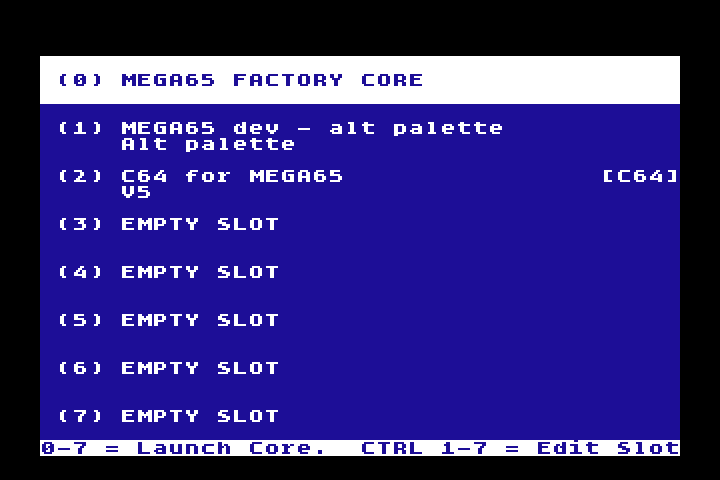
\includegraphics[trim= 0  0 0 10mm,clip,width=0.7\linewidth]{images/ss-flashmenu.png}
\end{center}

To select a core and start it, use the cursor keys to highlight the desired core, and then press
\specialkey{RETURN}.  If you select a flash slot that does not
contain a valid core, it will be highlighted in red to indicate that it
cannot be booted from:

\begin{center}
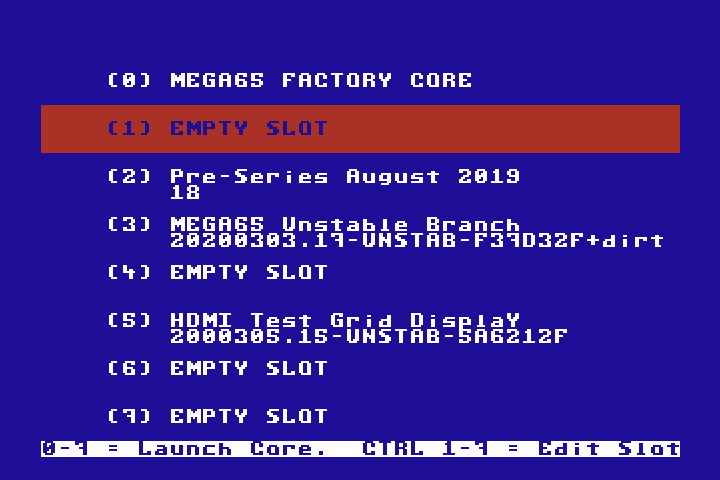
\includegraphics[trim= 0  0 0 10mm,clip,width=0.7\linewidth]{images/ss-flashmenu-invalidslot.png}
\end{center}

Alternatively, you can press the number corresponding to the core you would
like to use. The MEGA65 immediately reconfigures the FPGA, and launches the core.  If for some reason
the core is faulty, the MEGA65 may instead restart normally after a few seconds, and depending on the
circumstances, take you back into the menu automatically.

The MEGA65 will keep running the new core until you physically power it off.  Pressing the reset button
will not reset which core is being run.

\phantomsection
\section{Installing an Upgrade Core for the MEGA65}

Installing and upgrading the core (from a {\tt .cor} file) for the MEGA65 can be done in a few easy steps.

First, copy the core onto the MEGA65's SD card. You can do this by removing the SD card and copying a previously
downloaded core file to it from another computer. Alternatively,
you can insert an SD card that already contains the upgrade core. Finally, you can use the MEGA65 TFTP Server
program and the MEGA65's Ethernet port to upload the core upgrade file onto the SD card from another computer
on your local network.

The Flash Menu will use the external microSD slot over
the internal SD card, so if you have both a microSD card and SD card
inserted in your MEGA65, the Flash Menu will ignore the
internal SD card. To avoid this, simply copy the core(s) from the internal SD
card to the external microSD card, or temporarily remove the external
microSD card from the rear of your MEGA65, so that the Flash Menu will
be able to find the core files.  Also note that the Flash Menu
currently only supports DOS-style 8.3 character filenames in UPPERCASE. If your
core files have a longer name, you will need to rename them when
copying them onto your microSD or SD card.

Next, once you have the upgrade core on the MEGA65's SD card, enter the Flash and Core Menu as above,
i.e., switch off the power, and hold \specialkey{NO SCROLL} down while switching the power on again.  When the Flash
and Core Menu appears, hold \specialkey{CTRL} down and press
\megakey{1} (or \specialkey{CTRL} and a different number, if you wish to replace the
contents of a different flash slot). The MEGA65
will present you with a list of core files that are on the SD card:

\begin{center}
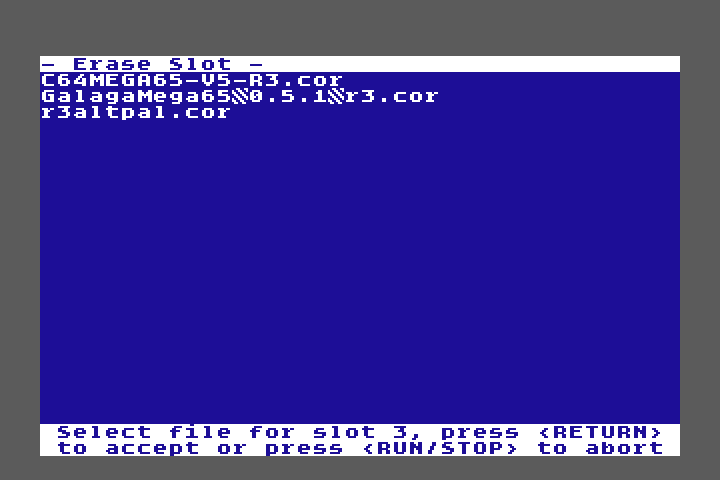
\includegraphics[trim= 10mm  5mm 10mm 15mm,clip,width=0.7\linewidth]{images/ss-flashmenu-selectcore.png}
\end{center}

Select the upgrade core file you wish to
install using the cursor keys, and then press \specialkey{RETURN}.  The MEGA65 will then erase
the flash slot, before writing the upgraded core.  You will see a progress bar while the MEGA65 erases
the flash slot:

\begin{center}
\includegraphics[trim= 10mm  3mm 10mm 15mm,clip,width=0.7\linewidth]{images/ss-flashmenu-erasing.png}
\end{center}

The progress bar will then reset, and the MEGA65 will
write the new core into the slot. This process can take up to 15
minutes, depending on the size of the core file.  If you simply wish
to erase a flash slot, you can select the
\screentext{-- erase slot --} option instead of a file name. This will then perform
only the erasure part of the process.

{\bf It is important to not switch the power off during this process}. If you do, the core file will be
only partially installed, and the MEGA65 may not start properly.
While
inconvenient, it won't damage your MEGA65 or leave it
in an unusable state: It will simply fall back to using the factory
supplied core.
If this happens, enter the Flash and Core Menu
as described above, and follow the instructions again.

When the flashing process has completed, you will see a message indicating that the process is complete:

\begin{center}
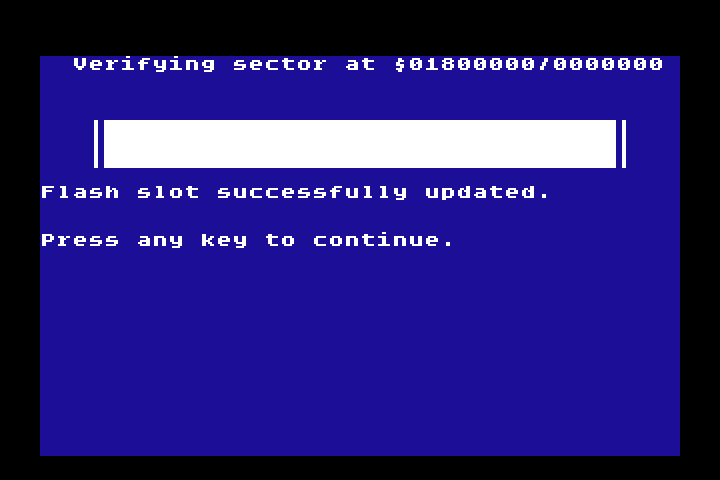
\includegraphics[trim= 10mm  3mm 10mm 15mm,clip,width=0.7\linewidth]{images/ss-flashmenu-done.png}
\end{center}


When this happens, simply switch off the power to the MEGA65 and switch it back on again for it to start using the
upgraded core.  This is because the MEGA65 will always try to start the core in slot 1 when
it is switched on.

\phantomsection
\section{Installing Other Cores}

Installing other cores works very similarly to installing upgrade cores. The only difference is that you
press \specialkey{CTRL} and \megakey{2} to \megakey{7} from the Flash and Core Menu, so that the core
gets installed to another slot.

Of course, there is nothing stopping you from installing a different core
in slot 1, so that the MEGA65 behaves as a different type of computer when you switch it on.  If you do this,
you can always choose to run the MEGA65 core by entering the Flash and Core Menu, and selecting the MEGA65
core.

\phantomsection
\section{Creating Cores for the MEGA65}

If you would like to create your own cores for the MEGA65, or help
contribute to the MEGA65 core, then
you may also wish to take a look at
\ifdefined\printmanual
the {\bf MEGA65 Book},
\else
\bookvref{cha:fpgacpldflashing},
\fi
which explains how to use the
FPGA development tools to flash the MEGA65.

\phantomsection
\section{Replacing the Factory Core in Slot 0}

Replacing the core in slot 0 is not recommended, because if it ever gets corrupted, it will ``brick'' the machine.
This will require you to connect a TE-0790 JTAG programmer, by opening your MEGA65 case, installing
the module, going through some rather convoluted software preparation steps (similar to if you were
creating your own bistream/core) and then restoring a working bitstream into the slot.

The MEGA65 is an open system though, so it's possible for you to do all of this, but it's very hard. There
is a secret key-press combination in the Flash Menu that will then challenge you with a series of questions with
increasing difficulty to ensure that you know what you are doing. Only after you have correctly
answered these questions will you be given the option to erase and/or replace the contents of slot 0.
Details of the questions asked are purposely not documented.

There really should be no reason for using this method to replace the contents of slot 0:
If you want to make your own bitstreams/cores, you can either write them to other slots and use the
Flash Menu to activate them, or you can simply use a TE-0790 JTAG programmer, and then use
Vivado or other FPGA development tool to write to the flash directly. This method is also
somewhat faster than flashing through the Flash Menu.

{\bf You have been warned!}

\phantomsection
\section{Understanding The Core Booting Process}

This section summarises how the MEGA65 selects which core to start with when it is switched on.
The process is shown in the following figure:

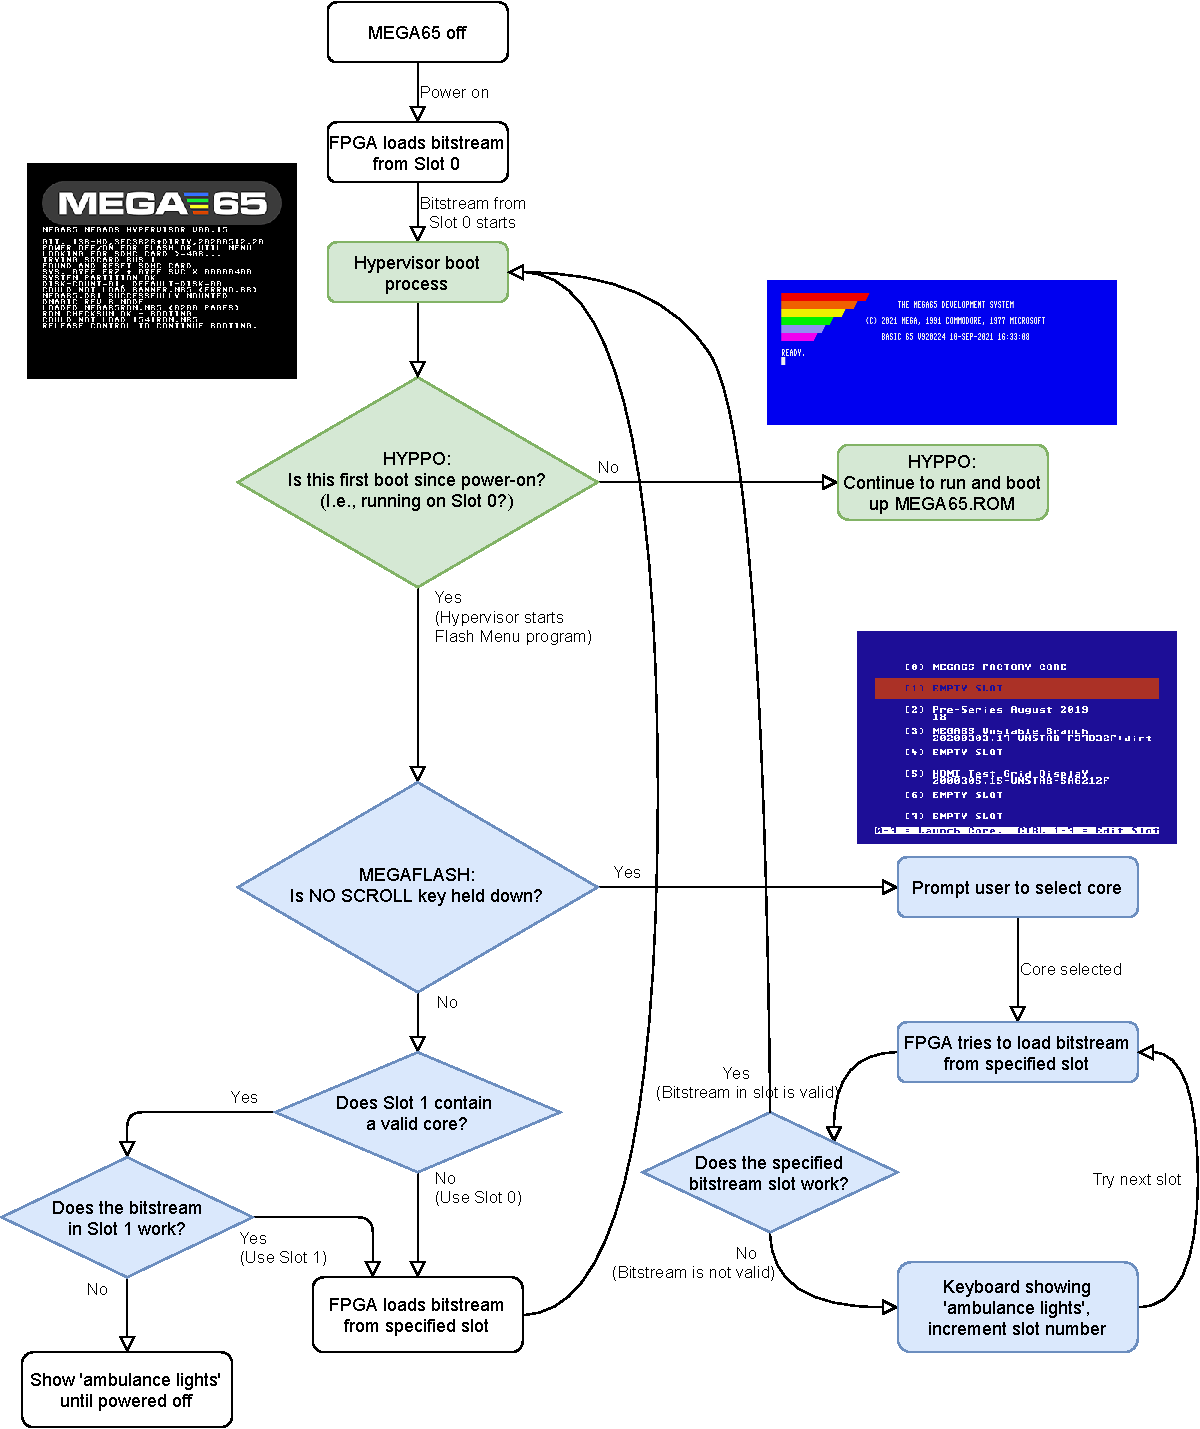
\includegraphics[width=\linewidth]{images/illustrations/flashmenu-flowchart.pdf}

The booting process is governed by two facilities:
\begin{itemize}
  \item The Hypervisor (also known as HYPPO), which operates at a level above the Kernal. One of its responsibilities is to manage aspects of the boot process. For more details on the Hypervisor, refer to  
\ifdefined\printmanual
the {\bf MEGA65 Book}.
\else
 \bookvref{sec:hypervisor-mode}.
\fi
    In the diagram, activities performed by the Hypervisor have been highlighted in green.
  \item The Flash Menu program (also known as MegaFlash), which provides a list of available core slots to choose from. In the diagram, activities performed by MegaFlash have been highlighted in blue.
\end{itemize}

When the MEGA65 is switched on, it does the following:
\begin{itemize}
\item Loads the bitstream stored in slot 0 of flash memory. If that is the MEGA65 Factory Core, the MEGA65 
  HYPPO Hypervisor starts.
\item If it is the first boot since power-on (which implies that we are running from slot 0), HYPPO starts the Flash Menu program (aka MegaFlash) -- but note that the Flash Menu in
      this mode may not show anything on the screen to indicate that it is running!
\item The Flash Menu then checks if \specialkey{NO SCROLL} is being held down.
\item If it is, the Flash Menu program shows its display, allowing you to select or re-flash a core.
\item If \specialkey{NO SCROLL} is \underline{not} being held down, the Flash Menu program checks if Flash Slot 1 contains a valid
      core.
\item If it does, then the Flash Menu program attempts to load that core.
\item If it succeeds, then the system reconfigures itself for that core, after which the behaviour of the system is
      according to that core.
\item If it fails, the keyboard will go into ``ambulance mode'', showing flashing blue lights to indicate that some
      first-aid is required. Note that in ambulance mode the reset button has no effect: You must switch the
      MEGA65 off and on again.
\end{itemize}



If you have selected a different core in the Flash Menu, the process
is similar, except that the ambulance lights will appear for only a
limited time, as the FPGA will automatically search through the flash
memory until it finds a valid core. If it gets to the end of the flash
memory, it will start the MEGA65 Factory Core from slot 0 again.

\phantomsection
\section{DIP Switches}

The MEGA65 motherboard has 4 DIP switches, some of which impact flashing and booting behaviour, so they are documented below:

\begin{center}
  \begin{longtable}{|L{1.5cm}|p{10cm}|}
    \hline
    {\textbf{Switch number}} & {\textbf{Purpose}} \\
    \hline
    1 & {Keyboard Flash enable/disable} \\
    \hline
    2 & {HDMI Audio enable/disable} \\
    \hline
    3 & {QSPI Flash enable/disable \newline
         Off = permit non-hypervisor access to QSPI flash. \newline
         On = disallow non-hypervisor access to QSPI flash.} \\
    \hline
    4 & {Boot Slot 0/1 select \newline
         Off = Boot from slot 0 \newline
         On = Boot from slot 1} \\
    \hline
  \end{longtable}
\end{center}
